\documentclass[a4paper,11pt]{report}
\usepackage[latin1]{inputenc}
\usepackage[english]{babel}
\usepackage{graphicx} 
\usepackage{pdfpages}
\usepackage{fancyvrb}
\usepackage{amsmath}
\newcommand{\argmax}{\operatornamewithlimits{argmax}}

\usepackage{cite}
\usepackage{url}
\bibliographystyle{unsrt}

\graphicspath{{images/}}
\begin{document}

\begin{titlepage}
\begin{center}

\includegraphics[width=5cm]{EURECOM_logo_quadri}
\\[3cm]
\textbf{\Huge{TBD}}
\\[2cm]
\textbf{\textsc{\LARGE{Semester Project Report}}}
\\[0.5cm]
\LARGE{Luca Venturini}
\\
\large{Spring 2013}
\\[8cm]
\columnsep3cm
\begin{tabular}{p{8cm} p{8.5cm}}
\small{\textbf{Supervisors:}\newline
Giuseppe Rizzo} \newline
Rapha\"el Troncy
&
\small{\textbf{EURECOM\newline Multimedia Department}}
\end{tabular}
\end{center}
\end{titlepage}

 \tableofcontents

\chapter{Introduction}
Natural Language Recognition studies how to allow a machine to understand and possibly interact with an human being by means of the word, without any other kind of interactions between the two. A sign, such as a word, is formed by a signifier and a signified; only the former, the word itself, is accessible to the machine, while the latter is something meaningful only for men. However, machines can store and elaborate information correlated to signifiers, as well as all the linkages between them, without the need to understand their meaning. In other words, a machine is useful whenever it can shorten the path linking two pieces of information and show to the man the final linkage, saving the time to go through all the path. Hence a machine can state the average life span for English monarchs, simply going through a knowledge base of historical figures and retrieving values for "age at death", without knowing the meaning of life or death (which would be problematic for men as well).

Usually a machine is able to work on structured data, i.e. where the pairs field-value and the relations are explicit, as in the previous example. The main goal of Natural Language Recognition is to retrieve information from unstructured data, as a news article or a free-text form. In the context of Web today, we see Petabytes of unstructured data "in the wild", and search engines which would like to index and understand some of the content enclosed in these pages; an effort to reach this result has been led by the promoters of Semantic Web, which attempts to have an uniform semantics over web pages dealing with the same topics, by means of tags (i.e. structured data "hidden" in the code of the page). However, too much unstructured information still exists to be manually structured by man.

\section{Named Entities}
A Named Entity is an entity which has a rigid designator, like a name (C.S. Lewis) or a number (year 1789). The definition of "rigid" can be loosened, depending on the task; sometimes money and time expressions are considered Named Entities as well, even in the cases they do not define uniquely a value (as in "at noon", when we don't know the 12 o'clock of which day we are talking about). Entities are named and unique even if they are not so in the text where they appear: in the sentence "The Queen died in 1603", "The Queen" is a designator for Queen Elizabeth I even if her name is not manifestly written, so a Named Entity Extractor should be defined to include such cases in the Named Entities.

Named Entity Extraction, also known as Named Entity Recognition (NER), and Named Entity Linking (NEL) are subtasks of Information Extraction. In NER, we want to extract all the entities cited in a document and recognize their type (such as Person or Organization). In NEL, we want to link a Named Entity (referred by the name by which it appears in the document and its position) to a node in a Knowledge Base (KB), e.g. Wikipedia. Together with Slot Filling, which allows to fill the values in the KB nodes from their unstructured description, this tasks form the bigger task of automatically building a Knowledge Base from raw data.

\section{The problem}
Named Entity Recognition needs a first phase of training: a big training set is needed to reach good results, data needs to be collected from various sources and labelled. The very first extractors were trained on articles from newspapers; but performances on different type of contexts (such as Web fora, narrative, email messages...) are much worse than on documents from the same type of source, or maybe the same newspaper.

The challenge here is to study how extractors can adapt to different contexts or corpora and how well they can react to the adaptation. In the next section, we will provide an insight on a NER system designed at Stanford, in order to give an understanding on how such training could be approached and what does it mean having a trained model. Next, we will look at TAC KBP evaluation campaign, where similar systems are compared and new trends for research in the field are proposed; we will focus particularly on NEL systems and their global performances, to have an idea on the evaluation method. Finally, we will present our web service, an interface to Stanford NER which allows an user to train it from own datasets.
%The final goal is to integrate it in a system which provides a single interface to many NER systems, NERD.

\chapter{State of the art}

\section{Conditional Random Fields}
\label{sec:crfs}
Conditional Random Fields (CRFs) were introduced by Lafferty, McCallum and Pereira in 2001\cite{lafferty2001conditional} as a probabilistic model to segment and label sequence data. Considering our Named Entity Recognition task as a subtask of the labelling problem, we can define a log-linear model
$$
p(\overline{y} \mid \overline{x}; w) = \frac{1}{Z(\overline{x}, w)}\exp\sum\limits_j w_jF_j(\overline{x}, \overline{y})
$$
where $\overline{x}$ and $\overline{y}$ are our training sequence and the respective label sequence, $w_j$ are real-valued weights for feature functions $F_j$ and $Z$ is a partition function, defined as
$$
Z(\overline{x}, w) = \sum\limits_{\overline{y}}\exp\sum\limits_j w_jF_j(\overline{x}, \overline{y})
$$
A model can contain hundreds of thousands of different feature functions, which are computed over a single word, its position in the sentence, its labelling and possibly all the surrounding context (the whole $\overline{x}$ and $\overline{y}$). As example, consider the word "A.C.M.E.": its punctuation and the capitalization are two features strongly suggesting we are talking about an organization.

Hence, training $w$ corresponds to the Maximum Likelihood Estimation of the parameters of our model, that is to say
$$
\hat{w} = \argmax_w p(\overline{y} \mid \overline{x}; w)
$$
Inference and decoding of $\overline{y}$ from a new sample $\overline{x}$ (i.e., labelling a document), will therefore correspond to
$$
\hat{y} = \argmax_y p(y \mid \overline{x}; \hat{w})
$$
There exist lots of methods to solve these two maximization problems in literature, and algorithms applied to the context of CRFs are still an interesting research field. Special training algorithms have been proposed, namely stochastic gradient ascent and derivations of Collins perceptron \cite{elkan2008log}.

\section{Stanford NER}
\label{sec:StfdNER}
Stanford NER \cite{finkel2005incorporating} is a Java implementation of Conditional Random Fields for Named Entity Recognition, coupled with good feature extractors. The software provides interfaces to access the main utilities by command line and APIs to control the classifier (also known as CRFClassifier, to disambiguate from other tools developed by the same university based on Hidden Markov Models).

The main difficulty approaching Stanford NER is the lack of documentation; little tutorials exist on using it by command line, but the only hints on APIs functioning are given by a couple of demos and the sourcecode itself.

The software allows to train the classifier from own data; as we have seen in Section \ref{sec:crfs}, we need some training data, i.e. a dataset of labelled documents. The input format makes the token-label pairs explicit by listing a token per line, as in the following example (where the character O stands for "Other"):


\begin{table}[h]
\begin{center}
\begin{tabular}{ll}
Sixteen &	O\\
years	& O\\
had	&O\\
Miss	&PERS\\
Taylor	&PERS\\
been	&O\\
in	&O\\
Mr.	&PERS\\
Woodhouse	&PERS\\
's	&O\\
family	&O\\

\end{tabular}
\end{center}
\caption{Input format for training datasets}
\label{tab:inputfmt}
\end{table}


Once a model for the classifier is trained, it cannot be modified; however, since the training is deterministic, it is still possible to create new instances of the classifier from scratch. Trained classifiers are serialized and compressed into an archive storing the necessary parameters to reload it.

Together with the library, Stanford provides already some good serialized classifiers, trained on 3 (Location, Person, Organization), 4 (Location, Person, Organization, Misc) and 7 Entity Types (Time, Location, Organization, Person, Money, Percent, Date), trained on CoNLL 2003 and MUC English training data. A typical use case sees the user loading these models from memory and elaborate some document, skipping the training part.

\chapter{Building a framework for NER adaptation}

%introduction and example of use
In this chapter, we will see how we developed a NER framework based on Stanford NER (Section \ref{sec:StfdNER}). The system provides a web interface which allows an user to train the classifier loading own datasets, and to use it on own documents. %TODO check this sentence
The web service is fully compliant to REST principles, %TODO footnote?
hence APIs are of easy access from a client implementing HTTP methods. 

\section{Profiling Stanford NER}
To design a service aimed to several users, able to manage different requests at the same time is not a trivial task. Performances of a NER system greatly vary accordingly to the input size (both for training and extraction) and can take the waiting time for the users over limits of bearability. Before approaching the whole design, we investigated on the bottlenecks of Stanford NER system, in order to understand which phases would have taken the biggest part in response time.

Tools used to profile Java code were the ones integrated in VisualVM \footnote{\url{http://visualvm.java.net}}.

\begin{figure}[htbp] 
\centering
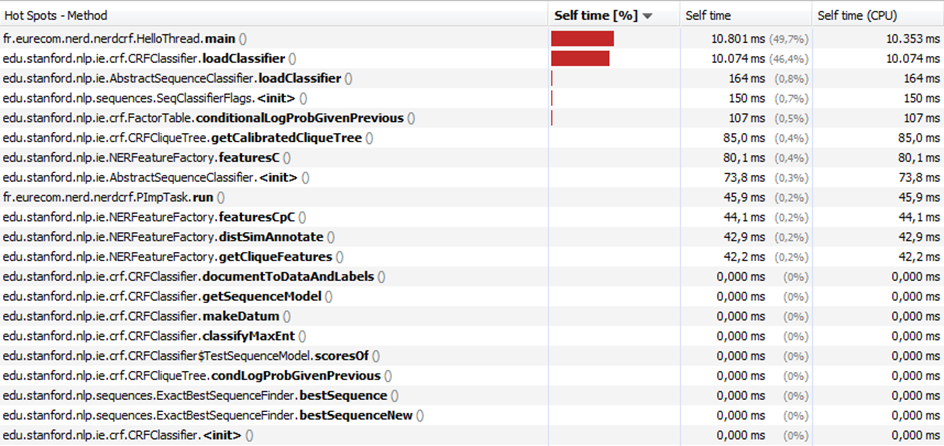
\includegraphics[width=\textwidth]{functions}
\caption{CPU usage per function call (small text)}
\label{fig:profile1}
\end{figure}

\begin{figure}[htbp] 
\centering
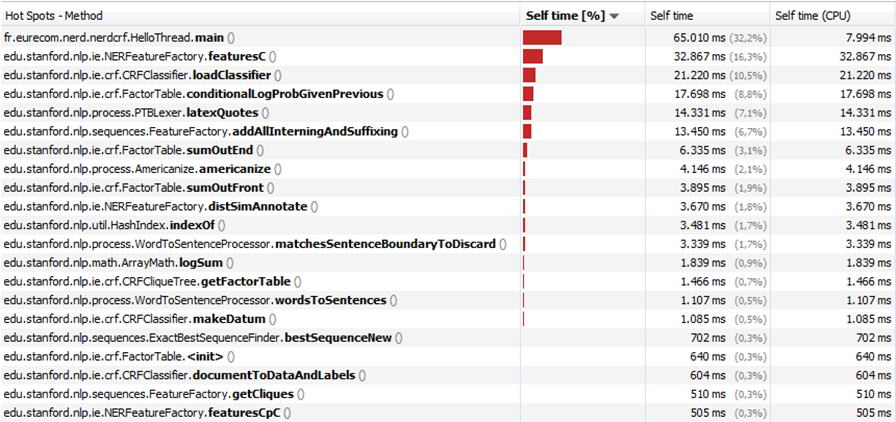
\includegraphics[width=\textwidth]{functions2}
\caption{CPU usage per function call (large text)}
\label{fig:profile2}
\end{figure}

We executed tests on a small text (the main content of a Wikipedia page)(Figure \ref{fig:profile1}) and on a bigger one, Jane Austen's Pride and Prejudice (Figure \ref{fig:profile2}).
As we can see in Figure \ref{fig:profile1}, the greatest part of the execution time is spent loading the model of the classifier from memory. As input size grows, the initial loading takes less percentage of the time, but it is still a remarkable load. In Figure \ref{fig:profile2} we notice also a second function taking a good slice of CPU time, \texttt{featuresC()}: this function is indeed in charge of tokenizing the text.

This data clearly show the need for avoiding unnecessary loads from disk: frequently used models should be kept in cache whenever possible, taking care of the hardware limits, since models can have great space requirements.

\section{Schema of resources}
%introduction to rest principles
Representational State Transfer (REST) is a software architecture style defined in 2000 by Roy Fielding and emerged as predominant design model for web APIs. %TODO cite Fielding?
In REST, client-server communication is based on the transfer of resource representations; therefore, we need to define what these resources are, how we identify them (URIs), by which HTTP method we can interact with them (GET, POST, PUT, DELETE) and which representation do we want for them.
Our system accepts requests for representations in XML or JSON.
Resources are the following (URI are given with relative path):
\subsection*{Documents}
The main collection for documents to be elaborated. Its URI is \texttt{/documents}.
Methods accepted:

\begin{description}
\item{POST} Create a new document, whose text is specified in the mandatory field \texttt{text}.
\end{description}

\subsection*{Document}
The document to be elaborated, i.e. whose entities we want to extract. Its URI is \texttt{/documents/\{doc\_id\}}.
Methods accepted:

\begin{description}
\item{GET} Get the representation for the document.
\end{description}

\subsection*{Annotations}
The main collection for results from extraction. Its URI is \texttt{/annotations}.
Methods accepted:
\begin{description}
\item{POST} Create a new annotation for document specified in field \texttt{id}, with the model specified in field \texttt{model} (optional). If model is not specified, the default one will be used.
\end{description}

\subsection*{Annotation}
The result from an extraction, a list of all entities recognized in the text. Its URI is \texttt{/annotations/\{ann\_id\}}. Methods accepted:
\begin{description}
\item{GET} Get the representation for the list of entity-label pairs.
\end{description}

\subsection*{Models}
The main collections for models. Its URI is \texttt{/models}. Methods accepted:
\begin{description}
\item{POST} Create a new model.
\end{description}

\subsection*{Model}
A model for Stanford classifier, i.e. a collection of training datasets. Its URI is \texttt{/models/\{mod\_id\}}. Methods accepted:
\begin{description}
\item{POST} Create a new training dataset for the model, from a file posted with content-type multipart/form-data, in CoNLL format (as in Table \ref{tab:inputfmt}). 
\end{description}

%TODO get for the training files?

\section{A sample use case}
%APIs
In the following scenario, an user tries the framework by submitting a document to the classifier with the default model; then, he repeats the experiment with a model self-trained, on a training set based on the first chapter of Jane Austen's Emma, where Named Entities of type Person are labelled.

The client used is \texttt{curl}\footnote{\url{http://curl.haxx.se}}.

\cleardoublepage
\addcontentsline{toc}{chapter}{Bibliography}
\bibliography{biblio}
\nocite{*}


\end{document}
